\chapter{The Domain Information Groper (dig)}

\section{Determine the authoritative DNS servers for the top level domain ru.}
Command: 
\textsl{ dig ns ru}
\begin{figure}[H]
\centering
  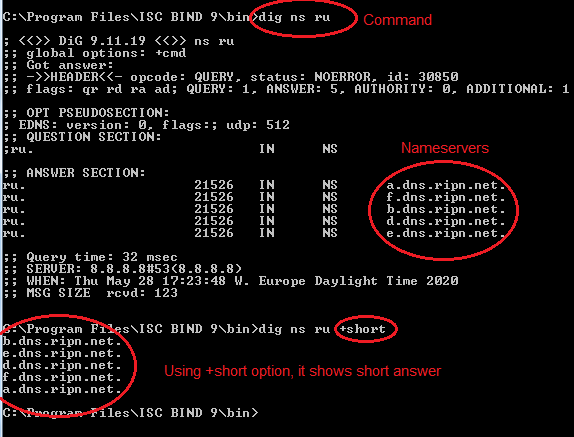
\includegraphics[width=0.6\textwidth]{Images/Image1-1-digTLD.png}
  \caption{dig command: DNS servers for "ru" TLD }
  \label{fig:1.1}
\end{figure}
\newpage
\section {Determine the addresses of the Internet DNS root servers.}
Command: 
\textsl{ dig ns .} 
\begin{figure}[H]
\centering
  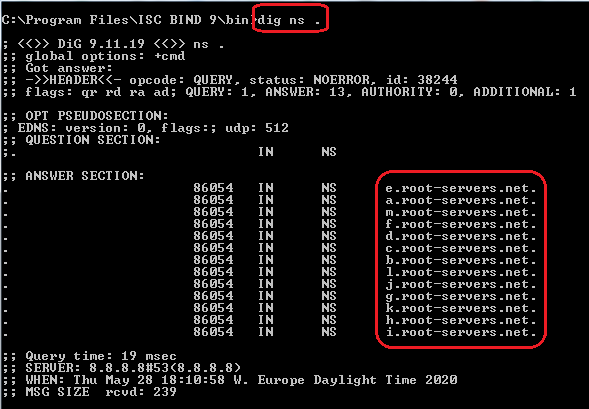
\includegraphics[width=.6\textwidth]{Images/Image1-2-DNSRoorServers.png}
  \caption{dig command: showing Internet DNS root servers}
  \label{fig:1.2}
\end{figure}
\section {Display the nameservers for the domain uni-bamberg.de}
Command: 
\textsl{ dig ns uni-bamberg.de } 

\begin{figure}[H]
\centering
  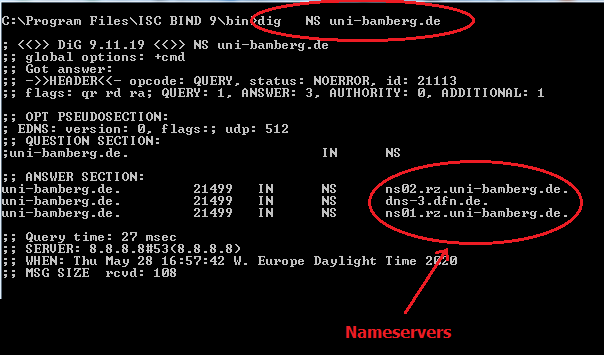
\includegraphics[width=.6\textwidth]{Images/Image1-3-digForaDomain.png}
  \caption{dig command: nameservers for a specific domain}
  \label{fig:1.3}
\end{figure}

\section{DIG}

\section{}

